\label{chp:anharmonicity}

As we have seen in the previous chapter, thermal conductivity is an anharmonic effect -- in a purely harmonic system, thermal conductivity is infinite. We have also discussed methods to assess thermal transport in materials, either via the Green-Kubo approach, or via perturbation theory, where the potential energy is expanded to third or fourth order, and these terms are used to compute the change of phonon properties, in particular, their lifetimes.\CITE{see paper}
From a computer simulation perspective, the two approaches have different strengths: Perturbative techniques are ideally suited, as the name suggest, when the anharmonicity is weak,~i.\,e.,~the harmonic terms in the potential dominate the dynamical evolution of the system. The Green-Kubo technique on the other hand does not need approximations to the potential energy surface, and therefore naturally includes all orders of anharmonicity. It is ideally suited in situations where the anharmonicity is strong,~i.\,e.,~when the basic assumption of perturbation theory is not satisfied. It is therefore desirable to \emph{measure} the ``degree of anharmonicity'', which, in turn, allows to discuss the question of anharmonicity not just in qualitative terms, but also in a quantitative way.

\newthought{The chapter is based on work performed by the author}, as published in Ref.\,\cite{Knoop2020}. We therefore only summarize the key ideas adopted in this work.\REM{say sth. else?}

\section{Definition of Anharmonicity}

In accordance with the previous chapters, the classical nuclear dynamics within Born-Oppenheimer approximation are governed by the Hamiltonian
\begin{align}
	\mathcal H ( {\bf P}, {\bf R}) 
		= \sum_I \frac{\b P_I^2}{2 M_I} + \mathcal V (\b R)~,
	\label{eq:anh.H}
\end{align}
where $\bf P$ and $\bf R$ denote the atomic momenta and coordinates, as usual. Using an expansion of the the full potential $\mathcal V {\bf R}$ in the displacements $\bf U$ as discussed in Chp.\,\ref{chp:dynamics}, the potential can be split into a harmonic contribution, $\mathcal V^{(2)}$, and a second term capturing all anharmonic effects, therefore termed $\mathcal V^{\rm A}$,
\begin{align}
	\mathcal V ({\bf R})
		= \mathcal V^{(2)} ({\bf R}) + \mathcal V^{\rm A} ({\bf R})~.
	\label{eq:anh.V}
\end{align}
In the classical limit, the dynamical evolution of the nuclei is determined by Eq.\,\eqref{eq:dyn.eom.classical},
\begin{align}
	M_I \ddot{\bf R}_I
		= -\frac{\partial \mathcal V}{\partial {\bf R}_I}
		\equiv {\bf F}_I~,
\end{align}
~i.\,e.,~in terms of the forces stemming from differentiating the potential. By linearity of the potential, the forces are therefore given by harmonic and anharmonic contributions as well,
\begin{align}
	{\bf F}_I
		= {\bf F}_I^{(2)} + {\bf F}_I^{\rm A}~.
	\label{eq:anh.F}
\end{align}
The division of potential and forces into harmonic and anharmonic contributions is depicted for a one-dimensional potential in Fig.\,\ref{fig:pes_sketch_vertical}.
\begin{marginfigure}
	\centering
	% 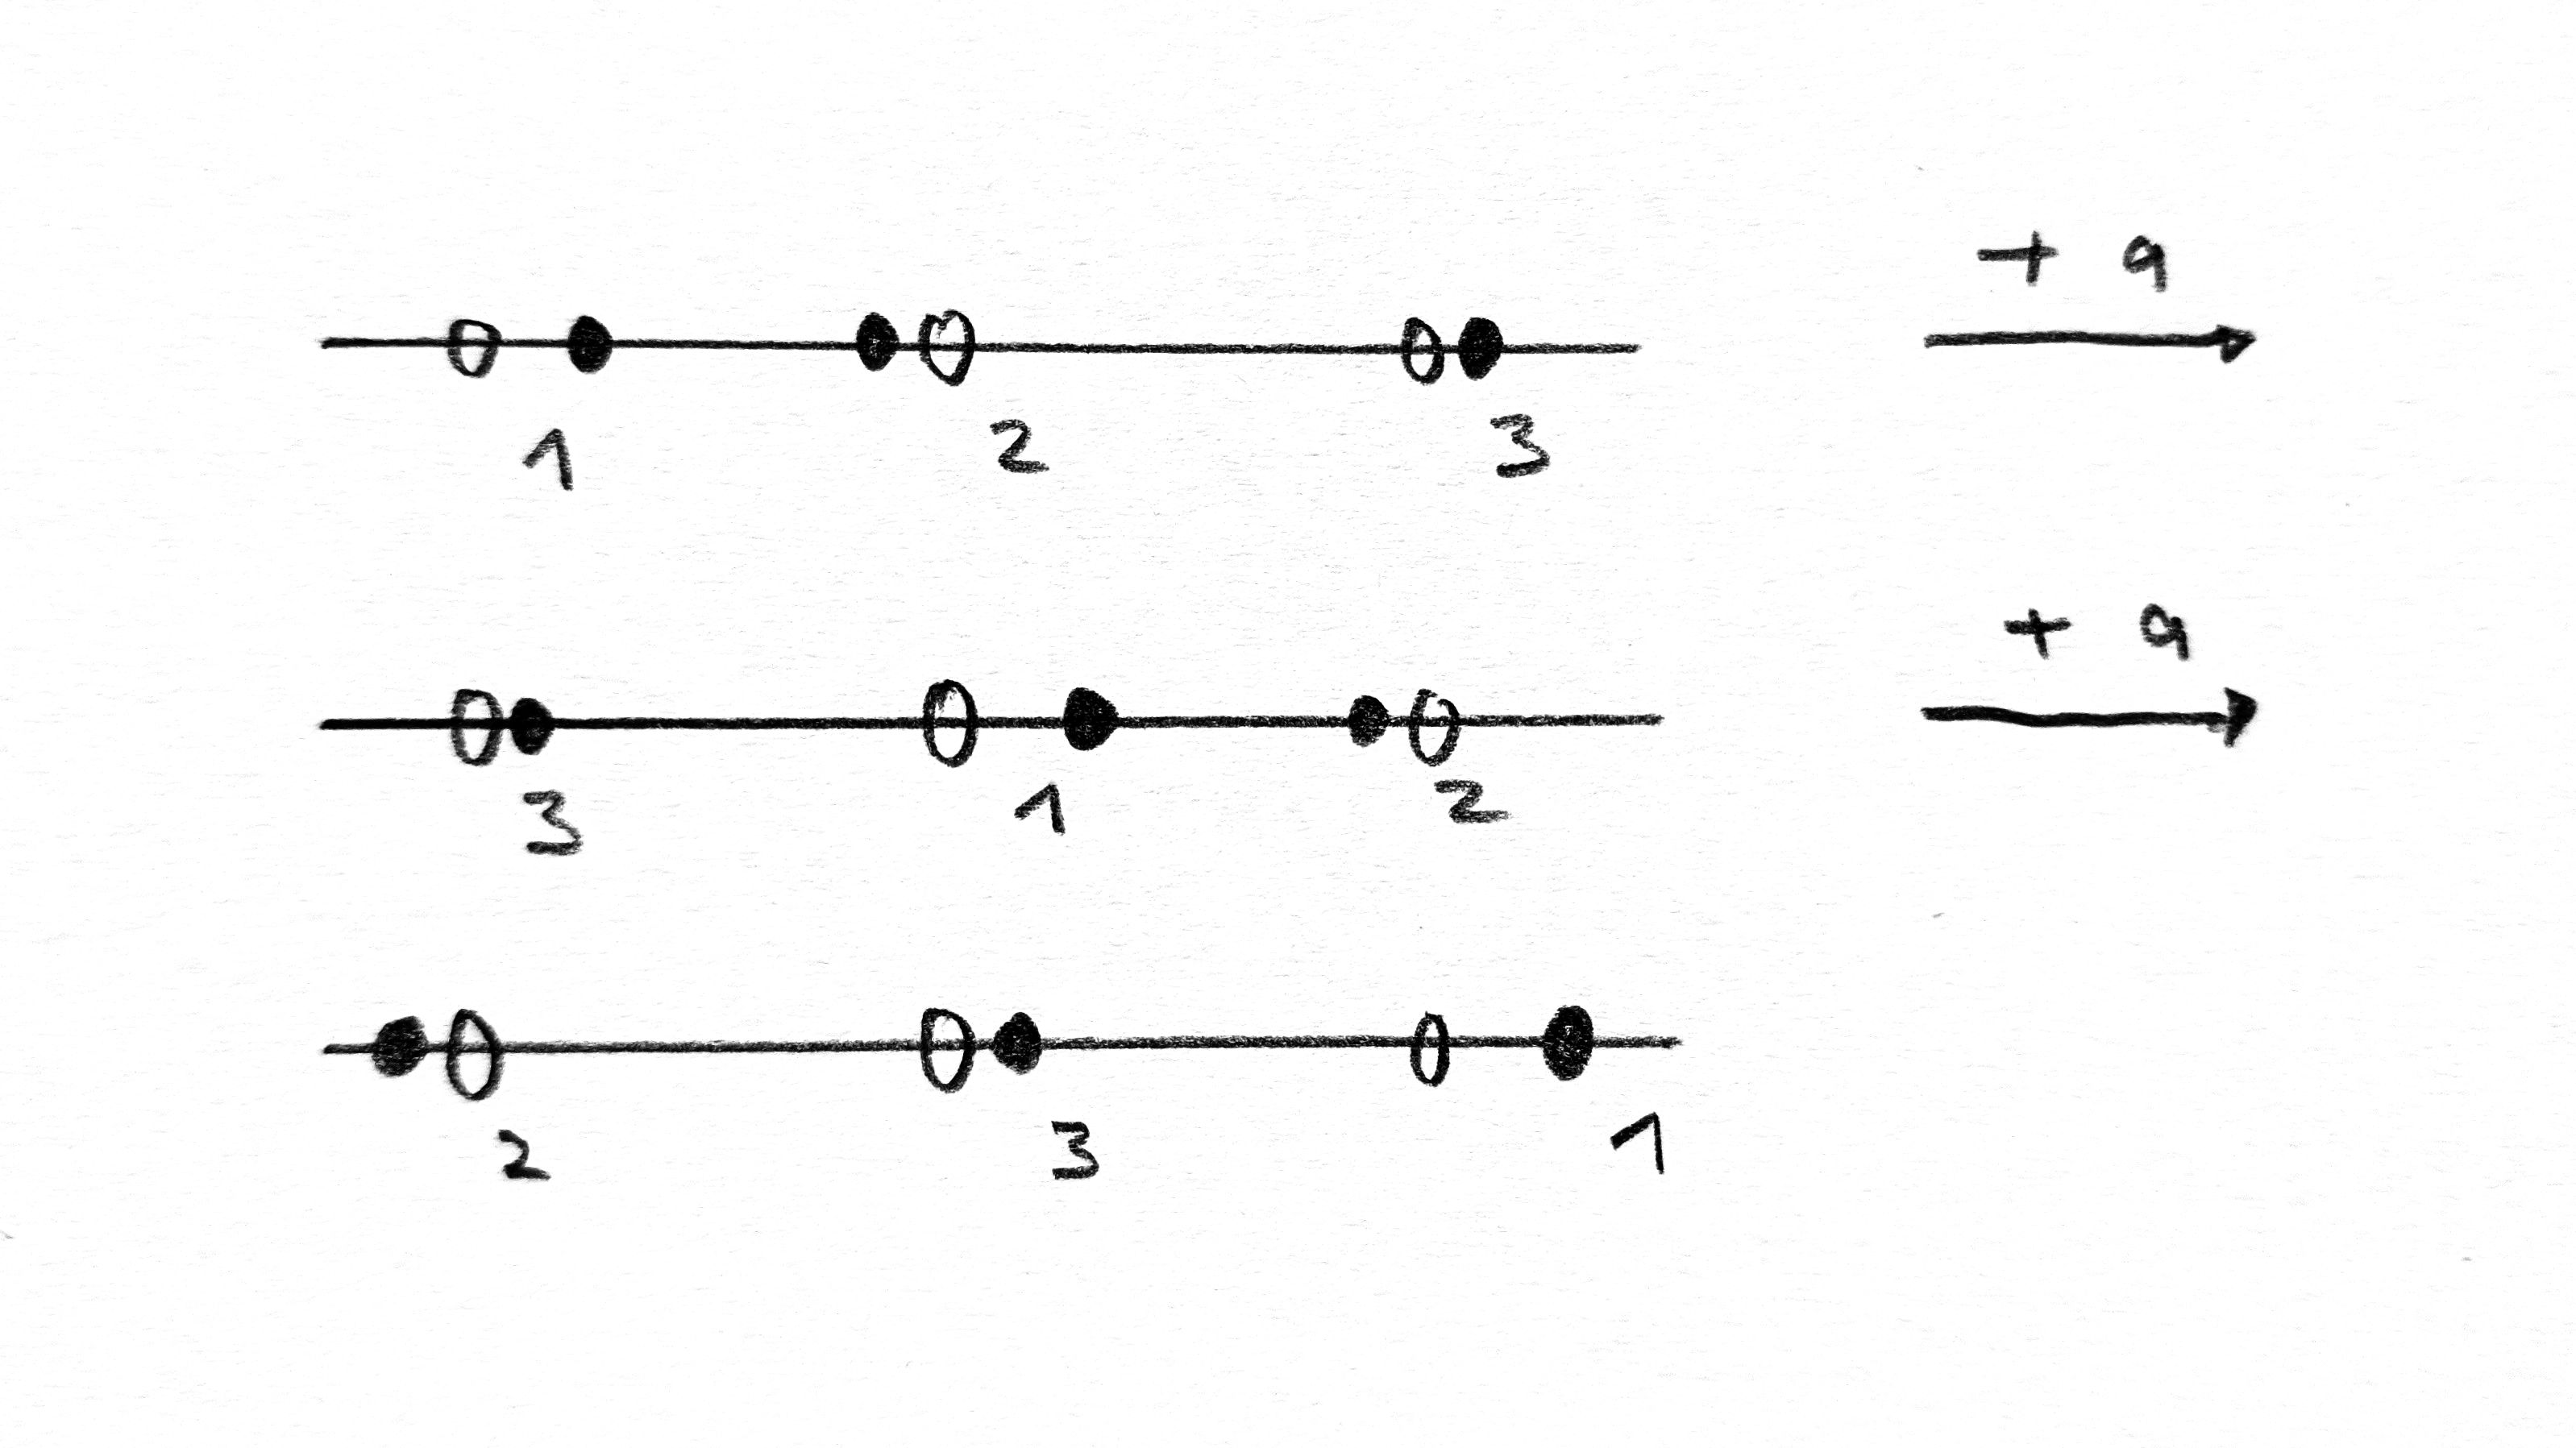
\includegraphics[width=.68\textwidth]{./sketches/permutation1.jpg}
	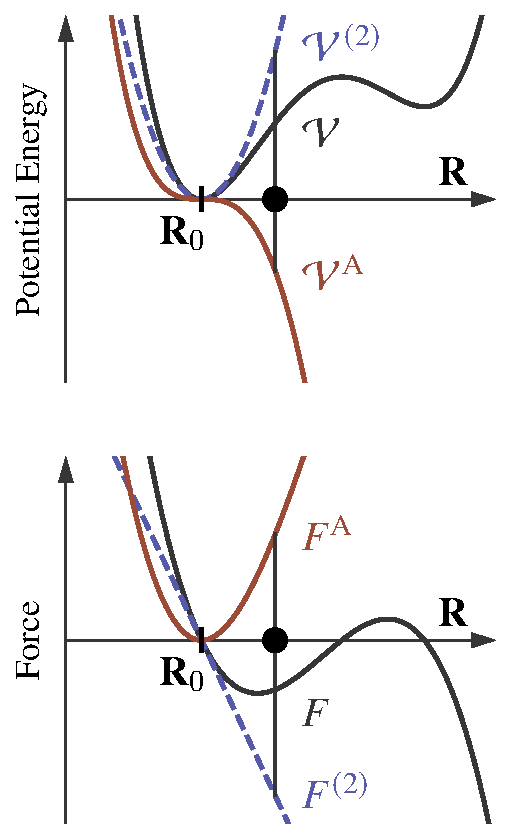
\includegraphics[width=\textwidth]{./data/plots/anharmonicity/1_pes_sketch/sketch_vertical.pdf}
	\caption{Upper: Sketch of a one-dimensional potential-energy surface $\mathcal V$ (solid black), its harmonic approximation $\mathcal{V}^{(2)} (\b R)$ (dashed blue), and the anharmonic contribution $\mathcal{V}^{\rm A} (\b R)$ (solid red). Right: The force ${F} ({\bf R})$ given by the derivative of the potential energy $\mathcal V$ (black), the force $F^{(2)}$ stemming from the harmonic potential $\mathcal{V}^{(2)} (\b R)$ (blue), and the anharmonic contribution $F^\mathrm{A} = F - F^{(2)}$ (red), cf.~Eq.\,\eqref{eq:anh.F}.}
	\label{fig:pes_sketch_vertical}
\end{marginfigure}


\section{Anharmonicity measure}

We base the discussion of anharmonicity in the following on the forces, for two reasons: First, because the dynamical evolution of the system is determined by the potential through the equations of motion, and therefore by the gradients,~i.\,e.,~the forces. Second, because the forces give more microscopic insight, as they can be resolved per atom, and better statistic, since per configuration $\bf R$, there are $3N$ force components ${\bf F} = ({\bf F}_1, \ldots, {\bf F}_N)$.

In terms of the force contributions defined in Eq.\,\eqref{eq:anh.F}, we define a \emph{measure of anharmonicity} in the following way:
\begin{align}
	\sigmaA (T)
		% = \frac{\sigma [F^{\rm A}]_T}{\sigma [F]_T}
		= \sqrt{\frac{\sum_{I, \alpha} \braket{(F^{\rm A}_{I, \alpha})^2}_T}{\sum_{I, \alpha} \braket{(F_{I, \alpha})^2}_T}}~,
	\label{eq:sigmaA}
\end{align}
where $F_{I, \alpha}^{(A)}$ is the $\alpha$ component of the (anharmonic) force on atom $I$, and $\braket{\cdot}_T$ denotes a thermodynamic average at temperature $T$. The interpretation of the measure $\sigmaA$ is that it quantifies the anharmonic strength in terms of the standard deviation of the distribution of anharmonic force components at a given temperature, $\sigma [F^{\rm A}]_T$, normalized by the standard deviation of the actual force distribution, $\sigma [F]_T$, where the standard deviation of force distributions is defined as
\begin{align}
	\sigma [F]_T 
		= \sqrt{\frac{1}{3N} \sum_{I, \alpha} \braket{F_{I, \alpha}^2}_T}~.
\end{align}
The effect of normalizing the distribution of forces is shown in Fig.\,\ref{fig:anh.normalization} for two exemplary materials, fcc-silicon, and an orthorombic perovskite, KCaF$_3$~\CITE{KCaf papers}.
\begin{marginfigure}
	\centering
	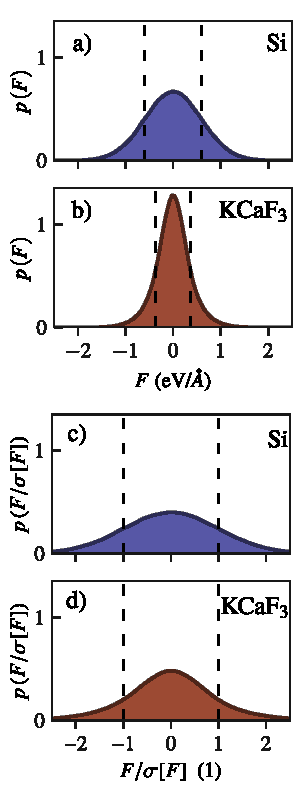
\includegraphics[width=0.8\textwidth]{./data/plots/anharmonicity/4_force_distribution/histogram_forces_vertical.pdf}
	\caption{
		Force component distribution before and after normalization with the width of the distribution $\sigma [F]$. $p(F)$ denotes the probability to find a force component $F_{I, \alpha}$ of strength $F$ in the material. Panel a) and b) show the distribution before normalization, c) and d) after normalization. Dashed vertical lines denotes the standard deviation of the displayed distribution.
	}
	\label{fig:anh.normalization}
\end{marginfigure}


\section{Examples}


%\begin{marginfigure}
%	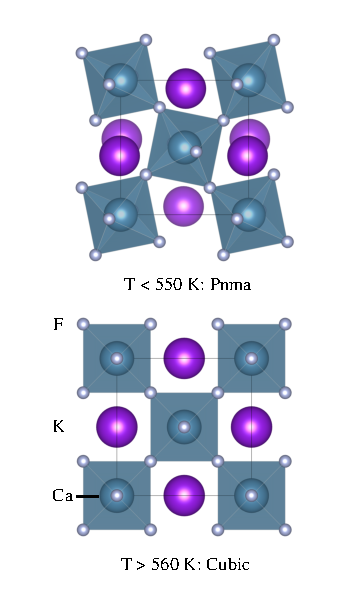
\includegraphics[width=\textwidth]{./data/plots/anharmonicity/2_materials/both.pdf}
%	\caption{
%		\label{fig:KCaF3}
%		KCaF$_3$ in the low-temperature Pnma~(left) and high-temperature aristotype phase~(right). Both structures are viewed along the long $b$-axis.
%	}
%\end{marginfigure}

\REM{Move to dynamics chapter?}
Silicon:


Visualize anharmonicity:

\begin{figure}
	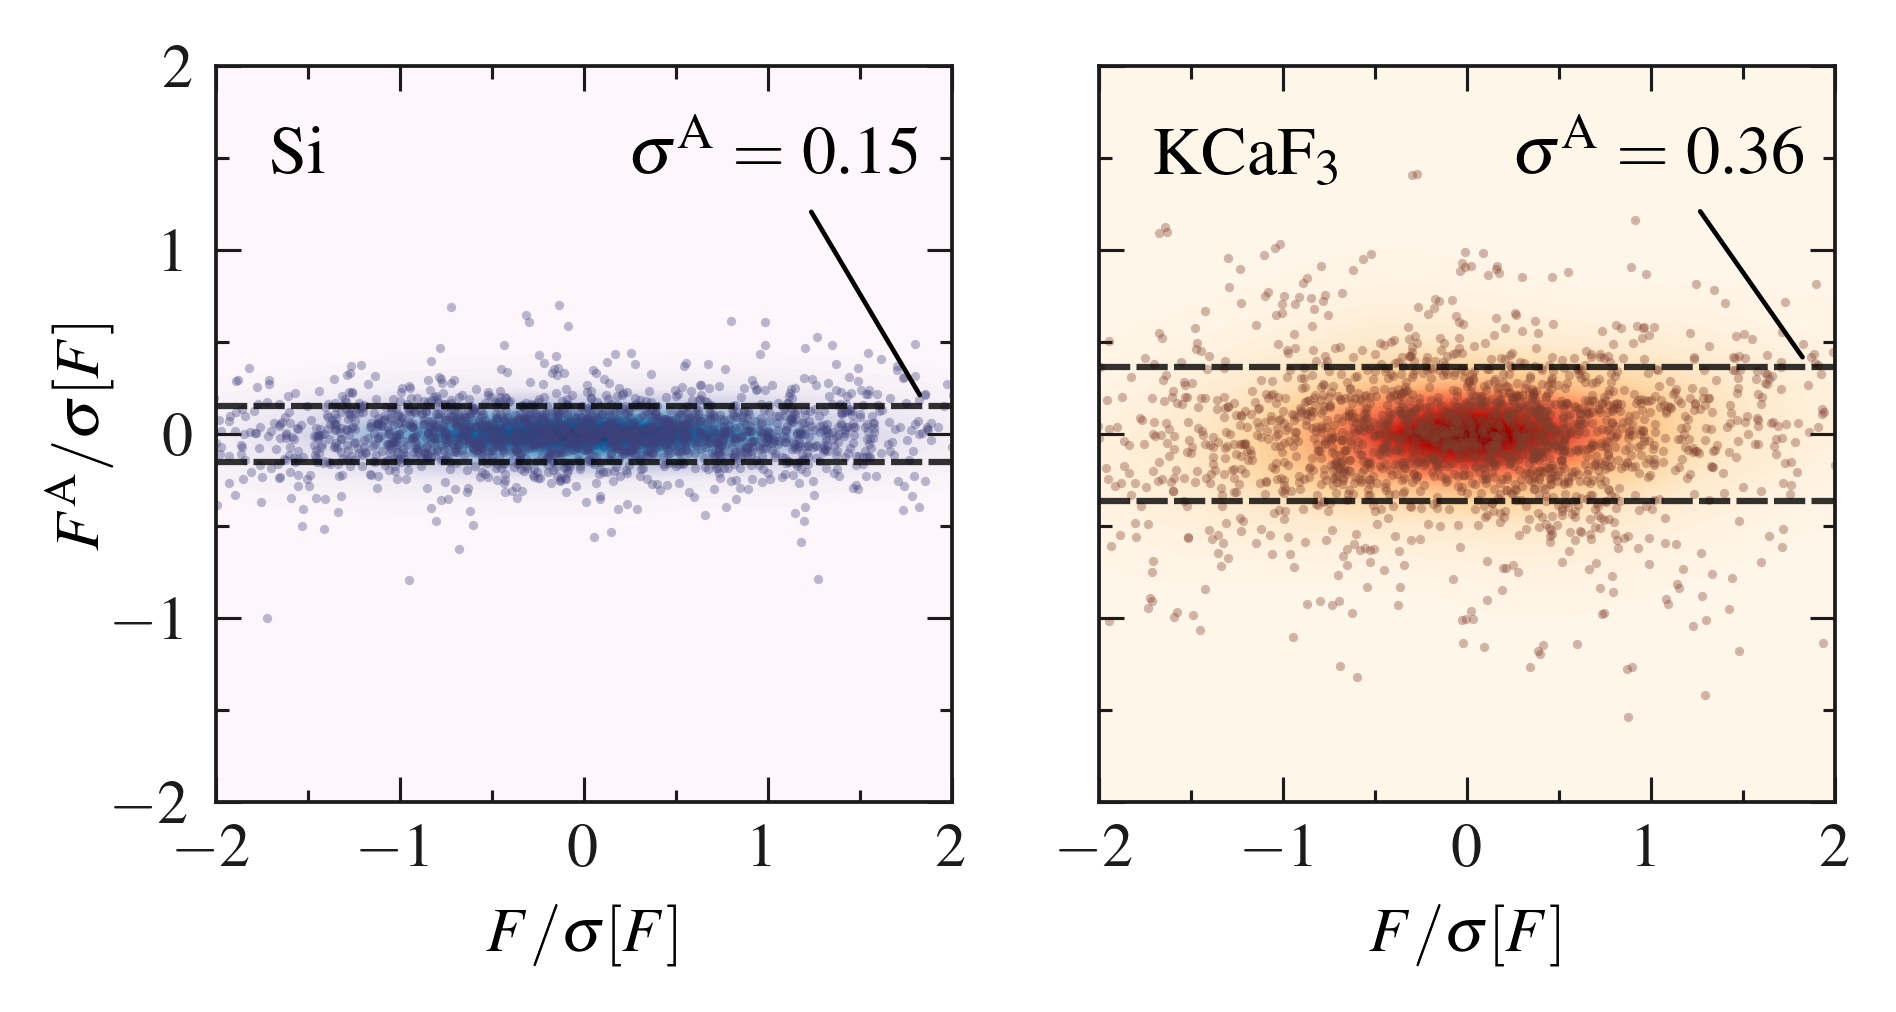
\includegraphics[width=\textwidth]{./data/plots/anharmonicity/5_density_plots/histogram_annotated.png}
	\caption{
		Normalized anharmonic force components versus normalized force components. Dashed horizontal lines: Width of the distribution estimated from standard deviation.
	}
\end{figure}

Anharmonicity can be analyzed for each atomic species in the material:

\begin{figure}
	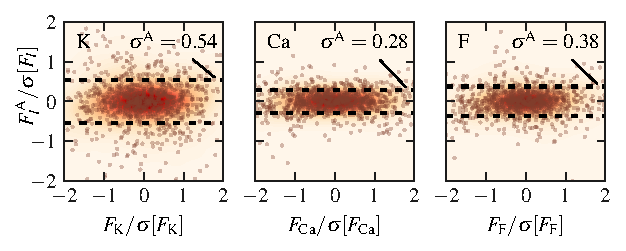
\includegraphics[width=\textwidth]{./data/plots/anharmonicity/5_density_plots/histogram_atoms.pdf}
	\caption{
		Normalized anharmonic force components versus normalized force components. Dashed horizontal lines: Width of the distribution estimated from standard deviation.
	}
\end{figure}

%
%\begin{figure}
%	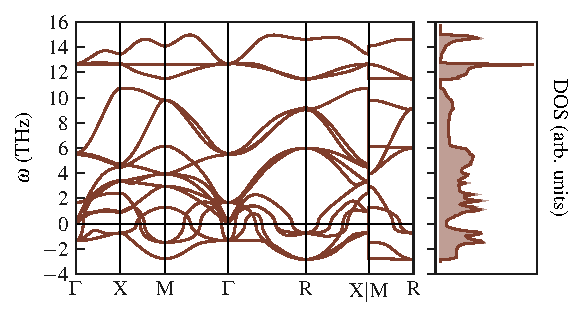
\includegraphics[width=\textwidth]{./data/plots/anharmonicity/3_bandstructures/KCaF3.cub/bands_dos_emb.pdf}
%	\caption{
%		Phonon bandstructure of KCaF$_3$ in the cubic structure obtained from a supercell with 160 atoms.
%	}
%\end{figure}
%
%\begin{figure}
%	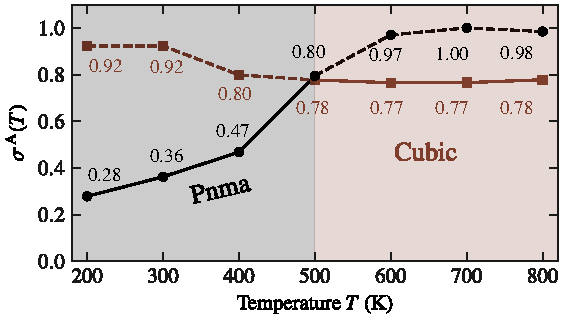
\includegraphics[width=\textwidth]{./data/plots/anharmonicity/6_phase_transition/sigma_temp_annot.pdf}
%	\caption{
%		Normalized anharmonic force components versus normalized force components. Dashed horizontal lines: Width of the distribution estimated from standard deviation.
%	}
%\end{figure}

\section{Screening Material Space}

\subsection{Preparation: Efficient Sampling of Anharmonicity}

\begin{figure}
	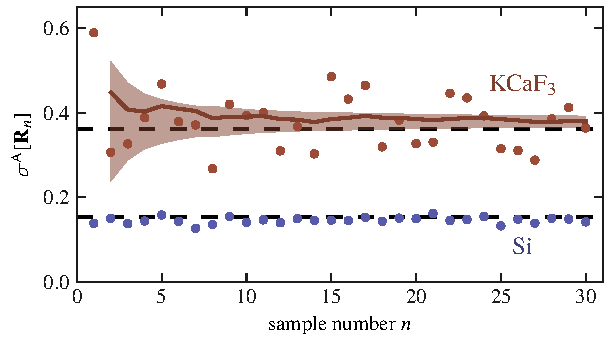
\includegraphics[width=4.1in]{./data/plots/anharmonicity/7_sampling/convergence_sigma_MC.pdf}
	\caption{
		Some text to describe the figure.
	}
\end{figure}

\begin{figure}
	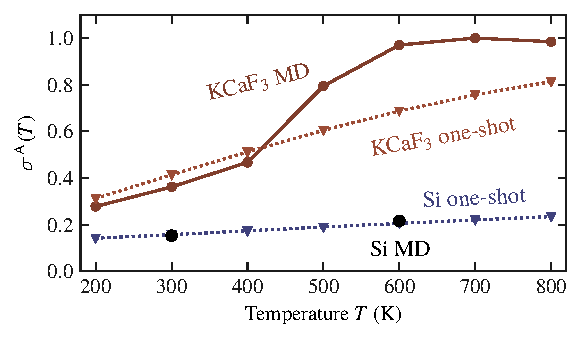
\includegraphics[width=4.1in]{./data/plots/anharmonicity/7_sampling/sigma_temp_one_shot.pdf}
	\caption{
		Some text to describe the figure.
	}
\end{figure}

\begin{figure}
	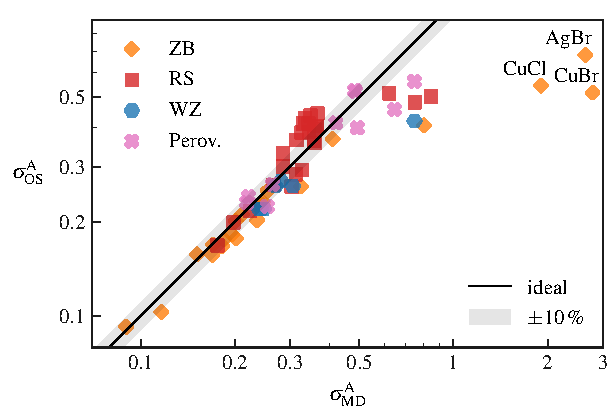
\includegraphics[width=4.1in]{./data/plots/anharmonicity/8_screening/sigma_os_md.pdf}
	\caption{
		Some text to describe the figure.
	}
\end{figure}

\subsection{Literature Review}


\begin{figure}
	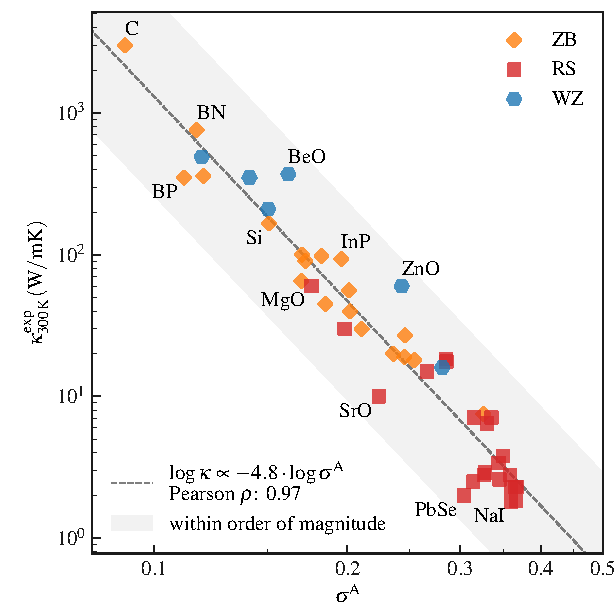
\includegraphics[width=4.1in]{./data/plots/anharmonicity/9_kappa/sigma_vs_kappa.pdf}
	\caption{
		Some text to describe the figure.
	}
\end{figure}



\subsection{Candidate Materials}